\documentclass[11pt,a4paper]{article}

\usepackage[margin=1in]{geometry}
\usepackage{booktabs}
\usepackage{array}
\usepackage{graphicx}
\usepackage{hyperref}
\usepackage{natbib}
\usepackage{tikz}
\usetikzlibrary{arrows.meta,positioning,fit}

\setlength{\parindent}{0pt}
\setlength{\parskip}{0.55em}
\renewcommand{\arraystretch}{1.08}

\title{A Hybrid Advanced AI Service for Quick Reorder Recommendation and Explainable Produce Quality Assessment}
\author{Advanced AI Coursework Draft}
\date{Academic Year 2025--26}

\begin{document}
\begin{titlepage}
\centering
\vspace*{1.5cm}

{\Large \textbf{Module Title: Advanced Artificial Intelligence}\par}
\vspace{0.3cm}
{\large \textbf{Module Code: UFCFUR-15-3}\par}
\vspace{0.3cm}
{\large \textbf{Academic Year: 2025--26}\par}

\vspace{1.8cm}
{\LARGE \textbf{A Hybrid Advanced AI Service for Quick Reorder Recommendation and Explainable Produce Quality Assessment}\par}

\vspace{1.2cm}
{\large Technical Report Draft\par}

\vspace{1.8cm}
\begin{tabular}{ll}
\toprule
\textbf{Student ID} & \textbf{Name} \\
\midrule
23085491 & Bui Vu Nhat Minh \\
Student ID 2 TBC & Member 2 Name TBC \\
Student ID 3 TBC & Member 3 Name TBC \\
\bottomrule
\end{tabular}

\vfill
{\large Bristol Regional Food Network AI Coursework Project\par}
\vspace{0.2cm}
{\large May 2026\par}
\end{titlepage}

\section{Problem Characteristics and Technical Challenges}
The BRFN case study requires an AI component that supports marketplace ordering and produce quality inspection. This is not only a modelling problem: the solution must operate as an independent Advanced AI service with HTTP interfaces, while remaining auditable for producers, customers and administrators \citep{uwe_ai_spec_2026,uwe_case_study_2026}. The system has two streams. Task 1 recommends quick reorder and discovery products from purchase history. Tasks 2--4 classify fruit and vegetable freshness, map predictions into quality decisions, and expose explainable outputs through an API.

The first challenge is data realism. No real BRFN purchase history was available, so Task 1 uses a synthetic marketplace seed export containing 80 customers, 12 producers, 60 products, 483 orders and 1,794 order lines. This validates schema, ranking logic, fairness checks and integration, but may not represent real seasonal shocks, stock-outs, restaurant bulk orders or community-group behaviour. The recommender is not presented as a production-validated personalisation model.

The second challenge is label mismatch. The image dataset supports 28-way classification of 14 produce categories under healthy/rotten variants; it does not contain expert Grade A/B/C, physical size, ripeness percentage, defect-mask or bounding-box labels. The implemented CV component performs image-level freshness/defect-state classification. It does not localise individual rotten regions with bounding boxes or segmentation masks.

The third challenge is operational risk. A false-fresh decision can affect food safety and trust more than an unnecessary manual review. The system is therefore framed as an AI-assisted decision service, not an autonomous food-quality authority.

\section{Candidate Approaches Considered}
\begin{table}[ht]
\centering
\small
\caption{Decision matrix for candidate approaches.}
\begin{tabular}{p{0.25\linewidth}p{0.32\linewidth}p{0.34\linewidth}}
\toprule
Approach & Considered for & Decision \\
\midrule
Global popularity & Quick reorder baseline and cold start & Kept as transparent baseline; weak personalisation and high producer-concentration risk. \\
\textbf{Frequency-recency} & Repeat purchase prediction & \textbf{Selected for quick reorder} because it is personalised, explainable and works with sparse synthetic data. \\
\textbf{Co-occurrence} & ``You may also like'' discovery & \textbf{Selected for discovery}; based on pairwise basket association \citep{agrawal1993association}. \\
Custom CNN & CV baseline & Kept as benchmark, not final due to lower transfer-learning robustness. \\
MobileNetV2 & Lightweight CV transfer learning & Useful deployment candidate; not final because EfficientNetB0 gave stronger risk-adjusted results \citep{sandler2018mobilenetv2}. \\
ResNet50 & Strong CV challenger & Retained as main challenger; higher macro F1 but more high-confidence errors \citep{he2016resnet}. \\
\textbf{EfficientNetB0} & Final CV classifier & \textbf{Selected final model} for accuracy, weighted F1, error confidence and deployment profile \citep{tan2019efficientnet}. \\
YOLO/object detection & Defect localisation & \textbf{Rejected} for this submission because no bounding-box or defect-mask labels exist. \\
\bottomrule
\end{tabular}
\end{table}

For Task 1, a deep recommender or black-box ranker was considered but rejected as the core method. Public grocery datasets would provide scale, but their customer, product and producer identifiers would not match the companion marketplace data contract, while the local synthetic export preserves the integration interface. Training a complex model on small synthetic behaviour would overstate evidence. The accepted design therefore separates convenience from discovery: frequency-recency generates quick reorder candidates, while market-basket co-occurrence recommends related products not previously purchased where possible.

For Tasks 2--4, the project compared a custom CNN, MobileNetV2, EfficientNetB0 and ResNet50 with fine-tuning. ResNet50 remains the strongest challenger because residual learning supports deeper visual features \citep{he2016resnet}. EfficientNetB0 was selected not because it dominated every metric, but because it gave the best operational trade-off: marginally highest accuracy/weighted F1, substantially fewer high-confidence errors than ResNet50, and a lighter deployment profile. This makes model choice a risk-based engineering decision rather than a single-metric ranking.

\section{Design Choices and Hybrid Architecture}
\begin{figure}[ht]
\centering
\small
\resizebox{\textwidth}{!}{%
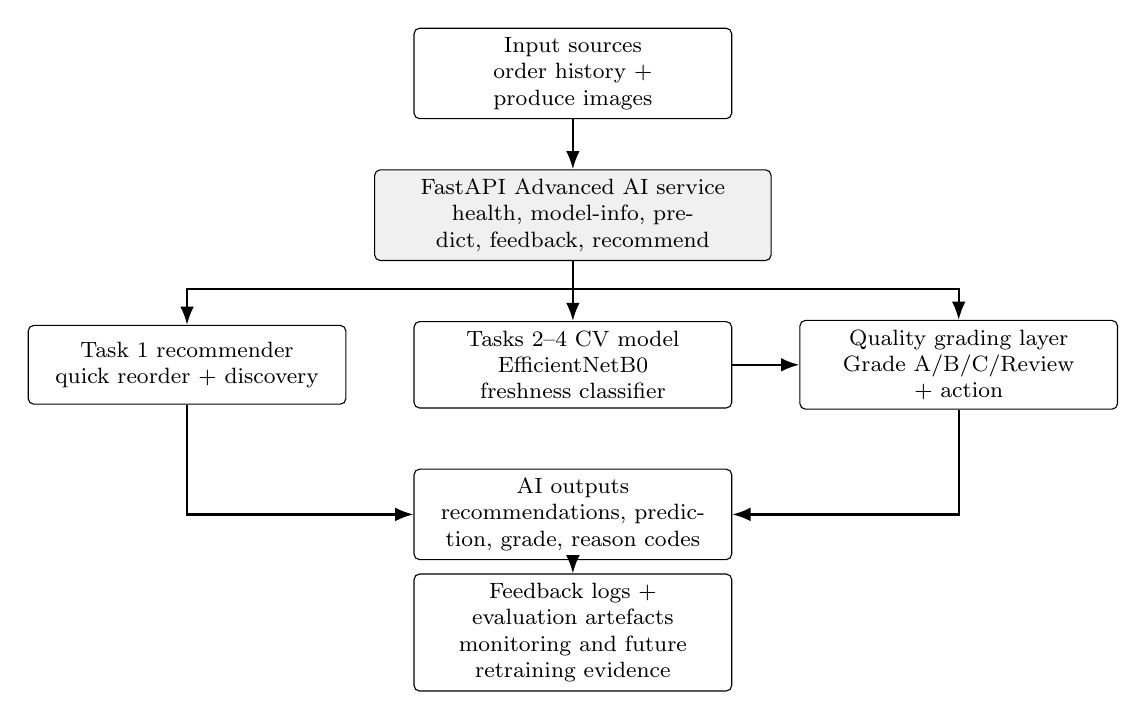
\begin{tikzpicture}[
  box/.style={draw, rounded corners=2pt, align=center, text width=3.8cm, minimum height=1.0cm, font=\footnotesize},
  service/.style={draw, rounded corners=2pt, fill=gray!12, align=center, text width=4.8cm, minimum height=1.15cm, font=\footnotesize},
  arrow/.style={-Latex, thick}
]

% High-level architecture for the Advanced AI service.
\node[box] (inputs) at (0,0) {Input sources\\order history + produce images};
\node[service] (api) at (0,-1.8) {FastAPI Advanced AI service\\health, model-info, predict, feedback, recommend};

\node[box] (rec) at (-4.9,-3.7) {Task 1 recommender\\quick reorder + discovery};
\node[box] (cv) at (0,-3.7) {Tasks 2--4 CV model\\EfficientNetB0 freshness classifier};
\node[box] (quality) at (4.9,-3.7) {Quality grading layer\\Grade A/B/C/Review + action};

\node[box] (outputs) at (0,-5.6) {AI outputs\\recommendations, prediction, grade, reason codes};
\node[box] (monitor) at (0,-7.1) {Feedback logs + evaluation artefacts\\monitoring and future retraining evidence};

\draw[arrow] (inputs) -- (api);
\draw[arrow] (api.south) -- ++(0,-0.35) -| (rec.north);
\draw[arrow] (api) -- (cv);
\draw[arrow] (api.south) -- ++(0,-0.35) -| (quality.north);
\draw[arrow] (cv) -- (quality);
\draw[arrow] (rec.south) |- (outputs.west);
\draw[arrow] (quality.south) |- (outputs.east);
\draw[arrow] (outputs) -- (monitor);
\end{tikzpicture}
}
\caption{Implemented Advanced AI service architecture. The service consumes order-history data and produce images, then returns recommendations, predictions, quality decisions, explanations and feedback/evaluation evidence through HTTP-facing components.}
\end{figure}

The recommender pipeline consumes five normalised CSV files: customers, producers, products, orders and order items. A temporal split evaluates whether products recommended from earlier purchases appear in later purchases. The live API uses all available historical orders and returns recommendation reason codes. Quick reorder uses frequency, recency, customer-type affinity and seasonality; discovery builds pairwise co-occurrence from baskets and applies diversity-aware re-ranking. Producer-facing outputs include week-level demand trends and a next-week forecast table for charting expected demand, for example rising or falling product quantities by producer. These are descriptive trend/forecast artefacts from synthetic order history, not a production forecasting model.

The computer-vision pipeline uses the final EfficientNetB0 artefact and class-name metadata to infer produce type and healthy/rotten condition from 224x224 images. Because the dataset cannot supervise Grade A/B/C, grading is handled by a separate transparent rule layer. The default score is:

\[
Q = 0.45M + 0.25C + 0.15D + 0.10I + 0.05S
\]

where \(M\) is model condition confidence, \(C\) is HSV colour-profile match, \(D\) is defect absence proxy, \(I\) is blur/brightness image quality and \(S\) is foreground area size proxy. The low weight on \(S\) is intentional because a single 2D image cannot measure physical size without calibration.

Safety gates run before normal grading. Confidence below 0.60 maps to Review. Rotten predictions with confidence at least 0.80 map to Grade C. Grade A requires a healthy prediction, model/color/size/ripeness/overall thresholds to be met, and no critical warning. Grade B covers acceptable healthy cases not meeting A, while Grade C also covers high dark ratio, low ripeness, low colour or low overall quality. FastAPI exposes `/health`, `/model-info`, `/predict`, `/feedback`, `/monitoring/feedback-summary` and `/recommend/reorder`; Docker Compose packages the service for repeatable demo deployment \citep{dockercompose2026}.

\section{Implementation, Testing and Evaluation}
The image pipeline was retrained with a grouped source-image split to reduce leakage from augmented variants of the same source image. The grouped split contains 19,674 training, 4,788 validation and 4,815 test examples, with zero overlapping source image IDs. This matters because a random split could inflate test performance if visually near-identical augmented images appear in both train and test.

\begin{table}[ht]
\centering
\caption{Computer-vision model comparison from the final confidence-audit notebook on the test set.}
\begingroup
\setlength{\tabcolsep}{5pt}
\renewcommand{\arraystretch}{1.32}
\footnotesize
\resizebox{\textwidth}{!}{%
\begin{tabular}{lrrrrrl}
\toprule
Model & Accuracy & Macro F1 & Weighted F1 & Total errors & High-conf. errors & Decision \\
\midrule
\textbf{EfficientNetB0 fine-tuned} & \textbf{0.97217} & 0.96138 & \textbf{0.97206} & \textbf{134} & 11 & \textbf{Final} \\
ResNet50 fine-tuned & 0.97155 & \textbf{0.96498} & 0.97152 & 137 & 19 & Main challenger \\
ResNet50 head & 0.96947 & 0.96150 & 0.96938 & 147 & 19 & Challenger \\
EfficientNetB0 head & 0.96656 & 0.95323 & 0.96639 & 161 & \textbf{9} & Head baseline \\
EfficientNetB0 XAI-corrected & 0.96386 & 0.95197 & 0.96373 & 174 & 17 & XAI check \\
MobileNetV2 fine-tuned & 0.95971 & 0.94407 & 0.95964 & 194 & 35 & Lightweight \\
MobileNetV2 head & 0.95182 & 0.93455 & 0.95194 & 232 & 27 & Lightweight \\
Baseline CNN + augmentation & 0.75036 & 0.68519 & 0.73923 & 1202 & 5 & Aug baseline \\
Baseline CNN + aug + oversample & 0.74746 & 0.71452 & 0.74213 & 1216 & 24 & CNN baseline \\
Baseline CNN & 0.73022 & 0.67371 & 0.72144 & 1299 & 6 & Initial baseline \\
\bottomrule
\end{tabular}
}
\endgroup
\end{table}

The final artefact is `models/best\_model.keras`, versioned in `models/model\_metadata.json` as `efficientnetb0\_aug\_oversampled\_finetuned\_wsl`, trained on the grouped split with targeted oversampling and fine-tuning of the last 30 layers. In the final confidence audit it achieved 0.97217 accuracy, 0.96138 macro F1, 0.97206 weighted F1, 134 errors and 11 high-confidence errors. Rotten macro recall was 0.94567 and rotten weighted recall was 0.95597. The weakest rotten classes were Bellpepper, Potato and Carrot, which should guide future data collection. Metrics use standard precision/recall/F1 definitions as implemented in scikit-learn \citep{sklearnmetrics2026}. Accuracy was not sufficient alone because false-fresh errors have higher operational cost.

Custom household-image validation and the corrected XAI audit are treated as deployment-risk probes, not statistically powered tests. They showed that real images can differ through background, lighting, scale and camera conditions, supporting manual-review thresholds, image-quality warnings and capture guidance.

Task 3 is implemented as a model-lifecycle and integration layer: external notebook training, exported model artefact and metadata, API loading, versioned prediction responses, `/feedback` logging, monitoring summaries and a future retraining dataset path. Accuracy over time is monitored as a human-feedback proxy: each prediction is logged with model version, confidence, class, grade and review flag; producer/admin feedback records whether the AI was accepted or overridden. The monitoring layer joins these records by `prediction\_id` and reports daily class-accuracy proxy, grade-accuracy proxy, override rate and high-confidence override count through `/monitoring/feedback-summary` and exported files. This is not a controlled test-set accuracy measure, because feedback can be sparse and biased, but it directly answers whether real interactions are revealing drift, weak classes or over-confident mistakes. Feedback does not automatically retrain the model during the demo because unverified overrides could introduce new bias.

\begin{table}[ht]
\centering
\small
\caption{Task 1 top-3 recommender evaluation on synthetic marketplace seed data.}
\begin{tabular}{llrrrr}
\toprule
Task & Method & P@3 & R@3 & HR@3 & Coverage/diversity \\
\midrule
Reorder & Global popularity & 0.1167 & 0.0589 & 0.3000 & 0.0500 / 0.1667 \\
Reorder & User frequency & 0.1167 & 0.0524 & 0.3000 & 0.9333 / 1.0000 \\
Reorder & \textbf{Frequency-recency} & \textbf{0.1222} & 0.0551 & 0.3000 & \textbf{0.9333 / 1.0000} \\
\midrule
Discovery & \textbf{Co-occurrence} & \textbf{0.1389} & \textbf{0.1171} & \textbf{0.3833} & 0.4333 / 0.8333 \\
Discovery & Segment popularity & 0.1222 & 0.0856 & 0.3333 & 0.4833 / 0.9167 \\
Discovery & Global popularity & 0.1056 & 0.0881 & 0.3000 & 0.1833 / 0.6667 \\
\bottomrule
\end{tabular}
\end{table}

Task 1 results are modest, but appropriate for sparse synthetic data. Frequency-recency was selected because it slightly improved Precision@3 while preserving high product coverage and full producer diversity across 12 producers. Co-occurrence was selected for discovery because it achieved the best HitRate@3 and perfect novelty for 60 eligible customers. Producer coverage, recommendation share and largest-producer share are reported because popularity bias can harm less visible suppliers \citep{klimashevskaia2024popularity}.

The producer-facing trend and forecast files aggregate weekly demand, three-week moving averages, trend direction and predicted next-week quantity. They can be visualised as producer forecast charts, satisfying the case-study requirement in a limited proof-of-concept form. The period is too short for ARIMA, LSTM or long-range demand claims, so the report frames these outputs as descriptive planning evidence rather than production forecasts.

Testing covered loader schema validation, temporal split, bounded metrics, cold-start fallback, reason codes, discovery exclusion of already purchased products, diversity re-ranking, API recommender compatibility, quality-rule thresholds, invalid image handling and feedback logging. The full pytest suite passed in the implemented repository. Threats to validity remain: synthetic Task 1 behaviour, Kaggle image bias, class imbalance, no supervised grade labels and domain shift from real producer-captured images. Dataset shift is a known deployment problem when training and deployment distributions differ \citep{quinonero2009datasetshift}; mitigation is confidence gating, manual review, capture guidance and feedback monitoring.

\section{Explainability, Legal, Ethical and Professional Issues}
Explainability is split between model attention and business decision explanation. Grad-CAM provides class-discriminative saliency for CNN predictions \citep{selvaraju2017gradcam}. In this project it is report-facing attention evidence used to audit whether the model focuses on plausible produce regions, background bias or high-confidence failures. It is not a segmentation mask and is not used to calculate quality grade.

The operational explanation comes from the API response: top-k predictions, confidence, top1/top2 margin, component scores, grade, action, reason codes, warnings and manual-review flags. Task 1 recommendations similarly return reason codes such as `frequently\_ordered\_by\_customer`, `ordered\_recently`, `commonly\_bought\_together` and `seasonally\_available`. This directly supports fairness, accountability and trust (FAT) because stakeholders can see why a recommendation, grade or manual-review flag was generated \citep{uwe_faq_2026}.

Fairness risks differ by pipeline. In Task 1, popularity methods may repeatedly expose already dominant producers, so the evaluation includes product coverage, producer diversity and recommendation share by producer. In Tasks 2--4, producers with poorer camera quality, lighting or backgrounds may receive lower quality scores. The system mitigates this through image-quality warnings, low-confidence review and capture guidance rather than silent rejection.

Privacy and accountability are also explicit. Task 1 uses anonymised IDs rather than names, emails, phone numbers or full addresses. The UK data protection principle requires personal data to be adequate, relevant and limited to what is necessary \citep{govukdataprotection2026}. Prediction and feedback logs include model version, prediction ID and override snapshot so decisions can be audited, but the prototype avoids automatic retraining from unverified feedback. Professionally, the system should be presented as decision support for BRFN staff and producers, not as certified food-safety inspection.

\section{Use of Generative AI}
Generative AI was used as engineering support, not as a source of unverified results. It supported report structure planning, identification of evaluation risks, documentation refactoring, FastAPI/Docker/notebook debugging, and drafting unit tests and API examples. It was also used to challenge whether the quality layer should claim supervised Grade A/B/C learning; that claim was removed because the dataset does not contain grade labels.

GenAI was not used to fabricate metrics, invent model results, replace final technical judgement or create fake evidence. All numbers in this report were checked against CSV/JSON artefacts such as `task1\_summary.json`, `recommender\_metrics.csv`, `discovery\_metrics.csv`, `final\_model\_metrics.json` and `model\_metadata.json`. Generated code and text were manually reviewed against the actual repository, then verified through notebook outputs, pytest, API curl responses and Docker tests.

The main limitation was overclaiming. Some generated suggestions implied object detection, defect localisation, calibrated physical size, automatic retraining or production recommendation accuracy. Those suggestions were rejected or rewritten. The final GenAI value was therefore not automatic content generation, but faster critical review and conversion of broad assessment risks into concrete tests, endpoints, documentation and report wording \citep{uwe_ai_spec_2026}.

\section{Recommendation and Conclusion}
The implemented system is suitable as a prototype AI decision-support service. Task 1 provides transparent quick reorder and discovery recommendations with producer-diversity evidence. Tasks 2--4 provide a strong image-level freshness classifier, conservative quality grading, XAI evidence, feedback logging and Dockerised API deployment.

It should not be deployed as an autonomous food-quality or production recommendation authority. Before real deployment, BRFN would need real transaction history, producer-uploaded image data, expert Grade A/B/C labels, calibration under varied cameras, retention rules for logs and a reviewed retraining process. The current contribution is a tested, explainable and integration-ready AI architecture.

\bibliographystyle{apalike}
\bibliography{references}

\clearpage
\appendix
\section{Appendix: Suggested Report Figures From Repository Artefacts}
The following figures are selected from existing notebook outputs. In Overleaf, upload these image files into the same folder as `main.tex` or adjust the paths to match the Overleaf folder structure.

\begin{figure}[ht]
\centering
\includegraphics[width=0.92\textwidth]{efficientnetb0_aug_oversampled_finetuned_wsl_training_curves.png}
\caption{Training and validation curves for the selected EfficientNetB0 fine-tuned model. Use this to evidence convergence and overfitting risk.}
\end{figure}

\begin{figure}[ht]
\centering
\includegraphics[width=0.92\textwidth]{efficientnetb0_aug_oversampled_finetuned_wsl_confusion_matrix.png}
\caption{Confusion matrix for the selected EfficientNetB0 fine-tuned model on the grouped test split. Use this to discuss weak classes and error concentration.}
\end{figure}

\begin{figure}[ht]
\centering
\includegraphics[width=0.92\textwidth]{resnet50_aug_oversampled_finetuned_wsl_confusion_matrix.png}
\caption{Confusion matrix for the ResNet50 fine-tuned challenger. Use this alongside EfficientNetB0 to justify model selection as a risk trade-off, not pure accuracy ranking.}
\end{figure}

\begin{figure}[ht]
\centering
\includegraphics[width=0.92\textwidth]{00_Banana__Rotten.png}
\caption{Grad-CAM model-comparison example for a rotten banana class. Use this to show model attention evidence, not defect segmentation.}
\end{figure}

\begin{figure}[ht]
\centering
\includegraphics[width=0.92\textwidth]{00_true_Bellpepper__Rotten_pred_Bellpepper__Healthy.png}
\caption{Failure-analysis Grad-CAM example: true rotten bell pepper predicted healthy. Use this as evidence for high-risk false-fresh analysis and manual-review safeguards.}
\end{figure}

\begin{figure}[ht]
\centering
\includegraphics[width=0.92\textwidth]{00_Bellpepper__Rotten.png}
\caption{Before/after XAI-corrected experiment example. Use this to discuss why the corrected experiment was analysed but not selected as final.}
\end{figure}

\begin{figure}[ht]
\centering
\includegraphics[width=0.92\textwidth]{05_mid_banana_model_comparison.png}
\caption{External/custom image validation example for a mid-quality banana. Use this to discuss domain shift, lighting, object scale and why the quality layer may require manual review.}
\end{figure}

\end{document}
